\graphicspath{ {images/student/} }

\section{Студенты}

Раздел \quotes{Студенты} содержит в себе функции по работе со студентами: загрузку студентов на Платформу, зачисление, 
отчисление, изменение режима прохождения сессии курса. Перейти в раздел можно, выбрав его в верхнем меню 
(см. рис. ~\ref{img:student:top_menu}).
\begin{figure}[H]
	\center{
\includegraphics[width=1\linewidth]{top_menu}}
	\caption{Раздел \quotes{Студенты}}
	\label{img:student:top_menu}
\end{figure}


\subsection{Роли и операции}
Раздел доступен пользователям роли \quotes{Администратор вуза}. Доступные операции:
\begin{itemize}
	\item в случае, если вуз является поставщиком и потребителем:
		\begin{itemize}
			\item загрузка студентов списком;
			\item просмотр студентов, обучающихся на курсах вуза;
			\item зачисление студентов;
			\item отчисление студентов;
			\item изменение режима прохождения;
			\item зачисление студентов списком;
			\item изменение режима прохождения списком;
			\item просмотр списка студентов вуза;
			\item просмотр подробной информации о студенте вуза;
			\item создание и редактирование заявки на зачисление;
			\item просмотр подробной информация о заявке на зачисление;
			\item создание заявки на изменение режима прохождения сессии курса;
			\item просмотр подробной информация о заявке на изменение режима прохождения сессии курса;
			\item создание заявки на зачисление;
			\item создание заявки на зачисление списком;
			\item создание заявки на изменение режима прохождения сессии курса;
			\item создание заявки на изменение режима прохождения сессии курса списком.
		\end{itemize}
	\item в случае, если вуз является только потребителем:
		\begin{itemize}
			\item загрузка студентов списком;
			\item просмотр списка студентов вуза;
			\item просмотр подробной информации о студенте вуза;
			\item создание и редактирование заявки на зачисление;
			\item просмотр подробной информация о заявке на зачисление;
			\item создание заявки на изменение режима прохождения сессии курса;
			\item просмотр подробной информация о заявке на изменение режима прохождения сессии курса;
			\item создание заявки на зачисление;
			\item создание заявки на зачисление списком;
			\item создание заявки на изменение режима прохождения сессии курса;
			\item создание заявки на изменение режима прохождения сессии курса списком.
		\end{itemize}
\end{itemize}


\subsection{Загрузка студентов списком}

Внешний вид формы загрузки студентов списком представлен на рис.~\ref{img:student:mass_invite}. 
Для осуществления загрузки студентов списком необходимо нажать на кнопку \quotes{Обзор} и в появившемся диалоге 
выбрать CSV"=файл в универсальном формате, рассмотренном в п.~\ref{sec:csv_format}. 

\begin{figure}[H]
	\center{
\includegraphics[width=1\linewidth]{mass_invite}}
	\caption{Загрузка студентов списком}
	\label{img:student:mass_invite}
\end{figure}

После выбора файла необходимо нажать на кнопку \quotes{Загрузить}, после чего начнется загрузка файла.
При загрузке файла без записей отобразится ошибка (см. рис.~\ref{img:student:empty_csv}).
\begin{figure}[H]
	\center{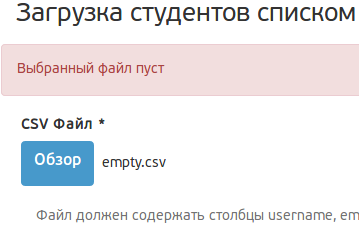
\includegraphics[height=3cm]{empty_csv}}
	\caption{Пустой CSV файл}
	\label{img:student:empty_csv}
\end{figure}

При загрузке корректного файла создается фоновая задача для его обработки и появляется соответствующее сообщение 
(см. рис.~\ref{img:student:invite_task_created}).

\begin{figure}[H]
	\center{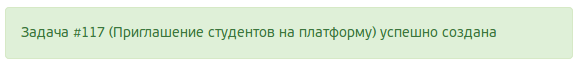
\includegraphics[height=1.5cm]{invite_task_created}}
	\caption{Сообщение о создании фоновой задачи}
	\label{img:student:invite_task_created}
\end{figure}

Для просмотра результатов выполнения задачи необходимо перейти в раздел \quotes{Фоновые задачи}, 
рассмотренный в п.~\ref{sec:mass_async_task}.

При загрузке студентов списком осуществляется набор проверок аналогичный рассмотренным в разделе 
приглашения сотрудника на Платформу  (см. п.~\ref{sec:invite}).
При нарушении этих проверок соответствующие ошибки появятся в результирующей CSV со списком неуспешно 
загруженных студентов.


\subsection{Обучающиеся на курсах вуза}
Список студентов, обучающихся на курсах вуза "--- это табличное представление всех студентов, 
проходящих обучение на какой"=либо сессии курса данного вуза.
Внешний вид списка представлен на рис.~\ref{img:student:enrolled_list}. 
Элементы управления табличными представления описаны в подразделе~\ref{sec:datatables}.
Таблица содержит следующие столбцы:
\begin{itemize}
	\item ФИО студента;
	\item адрес электронной почты;
	\item сессии курсов данного вуза, на которые зачислен студент;
\end{itemize}

\begin{figure}[H]
	\center{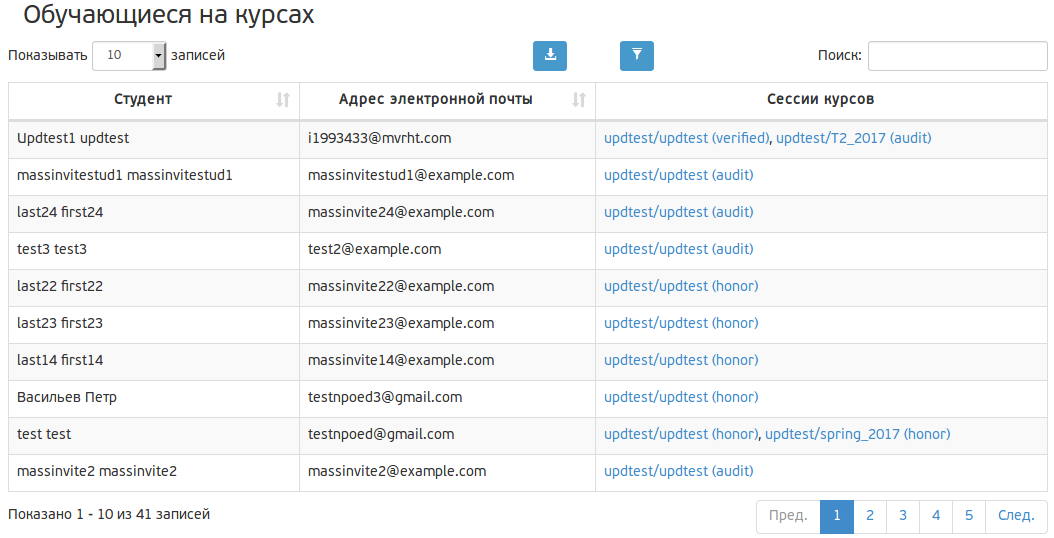
\includegraphics[width=1\linewidth]{enrolled_list}}
	\caption{Список студентов, обучающихся на курсах вуза}
	\label{img:student:enrolled_list}
\end{figure}

Внешний вид диалога фильтрации списка студентов представлен на рис.~\ref{img:student:enrolled_list_filter}.
Можно фильтровать список по следующим полям:
\begin{itemize}
	\item ФИО студента "--- текстовое поле;
	\item курс, на сессию которого он зачислен "--- виджет выпадающего списка с автодополнением с возможностью 
	множественного выбора (описание виджета см. в подразделе~\ref{widget:autocomplete_with_multiselect}).
\end{itemize}

\begin{figure}[H]
	\center{\includegraphics[height=5cm]{enrolled_list_filter}}
	\caption{Диалог фильтрации списка студентов, обучающихся на курсах вуза}
	\label{img:student:enrolled_list_filter}
\end{figure}

\subsection{Зачисление студентов}
Внешний вид формы зачисления студентов представлен на рис.~\ref{img:student:enroll}. 

\begin{figure}[H]
	\center{\includegraphics[width=1\linewidth]{enroll}}
	\caption{Зачисление студентов на сессию курса}
	\label{img:student:enroll}
\end{figure}

Для зачисления студентов необходимо:
\begin{enumerate}
	\item в выпадающем списке с автодополнением выбрать курс, который будут проходить студенты 
	(описание виджета см. в подразделе~\ref{widget:autocomplete});
	\item в выпадающем списке с автодополнением выбрать конкретную сессию этого курса 
	(описание виджета см. в подразделе~\ref{widget:autocomplete});
	\item в выпадающем списке с автодополнением выбрать один из режимов прохождения, доступных в рамках выбранной сессии 
	(описание виджета см. в подразделе~\ref{widget:autocomplete});
	\item опционально можно в выпадающем списке с автодополнением выбрать договор с вузом"=потребителем, 
	по которому осуществляется зачисление студентов (описание виджета см. в подразделе~\ref{widget:autocomplete});
	\item выбрать одного или нескольких студентов из числа уже зарегистрированных пользователей на Платформе при помощи 
	виджета выпадающего списка с автодополнением с возможностью множественного выбора 
	(описание виджета см. в подразделе~\ref{widget:autocomplete_with_multiselect}). 
\end{enumerate}

Изначально поля \quotes{Договор} и \quotes{Студенты} неактивны, они активируются только после выбора сессии курса.
После выбора курса в выпадающем списке сессий будут перечислены только сессии выбранного курса, 
а в списке договоров "--- только договоры, заключенные для этого курса, либо договоры без курсов.
После выбора сессии курса в списке студентов будут перечислены только студенты, 
которые еще не зачислены на выбранную сессию курса.

В случае, если заполнено поле \quotes{Договор} и количество свободных мест по договору меньше, 
чем количество выбранных для зачисления студентов, система выдаст предупреждение 
(рис.~\ref{img:student:enroll_student_error}), но на возможность зачисления студентов оно не влияет.

\begin{figure}[H]
	\center{\includegraphics[width=1\linewidth]{enroll_student_error}}
	\caption{Превышение количества студентов по договору.}
	\label{img:student:enroll_student_error}
\end{figure}

После заполнения всех полей необходимо нажать на кнопку \quotes{Зачислить}. Для зачисления студентов создается 
фоновая задача и появляется соответствующее сообщение (см. рис.~\ref{img:student:student_enroll_task}), 
а также осуществляется переход на список студентов, обучающихся на курсах данного вуза.
\begin{figure}[H]
	\center{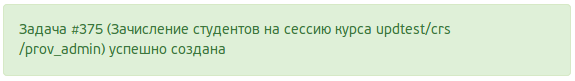
\includegraphics[height=1.5cm]{student_enroll_task}}
	\caption{Сообщение о создании фоновой задачи}
	\label{img:student:student_enroll_task}
\end{figure}

При зачислении для каждого выбранного студента осуществляются проверки:
\begin{itemize}
	\item студент не зачислен на выбранную сессию;
	\item если новый режим прохождения \quotes{verified} (с подтверждением личности), поле \quotes{Договор} 
	становится обязательным для заполнения; 
	\item если заполнено поле \quotes{Договор}, студент должен быть связан с вузом-потребителем из этого договора.
\end{itemize}

Для просмотра результатов выполнения задачи необходимо перейти в раздел \quotes{Фоновые задачи}, 
рассмотренный в п.~\ref{sec:mass_async_task}.

\subsection{Отчисление студентов}
Внешний вид формы отчисления студентов представлен на рис.~\ref{img:student:unenroll}. 

\begin{figure}[H]
	\center{\includegraphics[width=1\linewidth]{unenroll}}
	\caption{Отчисление студентов с сессии курса}
	\label{img:student:unenroll}
\end{figure}


Для отчисления студентов необходимо:
\begin{enumerate}
	\item в выпадающем списке с автодополнением выбрать курс, на который зачислены студенты 
	(описание виджета см. в подразделе~\ref{widget:autocomplete});
	\item в выпадающем списке с автодополнением выбрать конкретную сессию этого курса 
	(описание виджета см. в подразделе~\ref{widget:autocomplete});
	\item указать причину отчисления в текстовом поле; 
	\item выбрать одного или нескольких студентов из числа уже зарегистрированных пользователей на Платформе при помощи 
	виджета выпадающего списка с автодополнением с возможностью множественного выбора 
	(описание виджета см. в подразделе~\ref{widget:autocomplete_with_multiselect}). 
\end{enumerate}

После выбора курса в выпадающем списке сессий будут перечислены только сессии выбранного курса, 
а после выбора сессии курса в списке студентов будут перечислены только студенты, 
которые были зачислены на выбранную сессию.

После заполнения всех полей необходимо нажать на кнопку \quotes{Отчислить}. Для отчисления студентов создается 
фоновая задача и появляется соответствующее сообщение (см. рис.~\ref{img:student:student_unenroll_task}), 
а также осуществляется переход на список студентов, обучающихся на курсах данного вуза.
\begin{figure}[H]
	\center{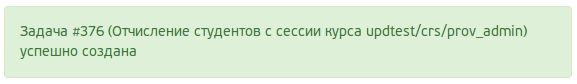
\includegraphics[height=1.5cm]{student_unenroll_task}}
	\caption{Сообщение о создании фоновой задачи}
	\label{img:student:student_unenroll_task}
\end{figure}

При отчислении для каждого выбранного студента осуществляются проверки:
\begin{itemize}
	\item студент был ранее зачислен на выбранную сессию;
	\item режим прохождения студентом сессии не равен \quotes{verified};
\end{itemize}

Для просмотра результатов выполнения задачи необходимо перейти в раздел \quotes{Фоновые задачи}, 
рассмотренный в п.~\ref{sec:mass_async_task}.

\subsection{Изменение режима прохождения сессии курса студентами}
Внешний вид формы изменения режима прохождения студентами сессии курса представлен на рис.~\ref{img:student:change_mode}.


\begin{figure}[H]
	\center{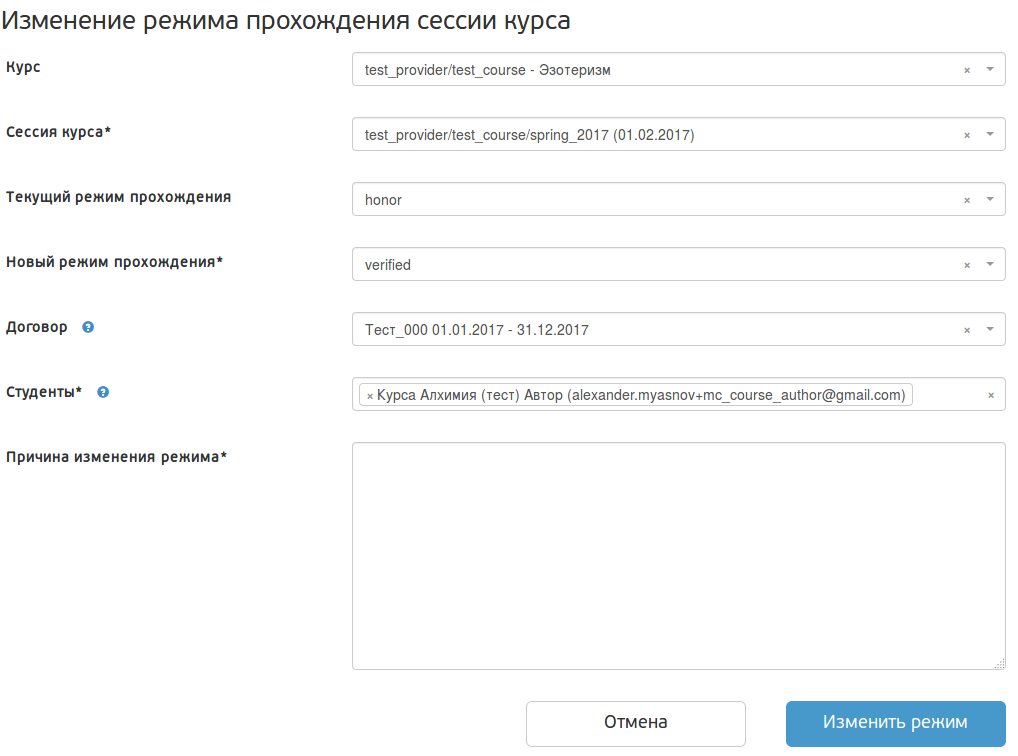
\includegraphics[width=1\linewidth]{change_mode}}
	\caption{Изменения режима прохождения студентами сессии курса}
	\label{img:student:change_mode}
\end{figure}

Для изменения режима прохождения студентами сессии курса необходимо:
\begin{enumerate}
	\item в выпадающем списке с автодополнением выбрать курс, на который зачислены студенты 
	(описание виджета см. в подразделе~\ref{widget:autocomplete});
	\item в выпадающем списке с автодополнением выбрать конкретную сессию этого курса 
	(описание виджета см. в подразделе~\ref{widget:autocomplete});
	\item опционально можно в выпадающем списке с автодополнением выбрать текущий режим прохождения среди 
	доступных в рамках выбранной сессии
	\item в выпадающем списке с автодополнением выбрать новый режим прохождения среди доступных в рамках выбранной 
	сессии, за исключением выбранного текущего режима (описание виджета см. в подразделе~\ref{widget:autocomplete});
	\item опционально можно в выпадающем списке с автодополнением выбрать договор с вузом"=потребителем, 
	по которому осуществляется зачисление студентов (описание виджета см. в подразделе~\ref{widget:autocomplete});
	\item выбрать одного или нескольких студентов из числа уже зарегистрированных пользователей на Платформе при помощи 
	виджета выпадающего списка с автодополнением с возможностью множественного выбора 
	(описание виджета см. в подразделе~\ref{widget:autocomplete_with_multiselect}). 
\end{enumerate}

Изначально поля \quotes{Договор} и \quotes{Студенты} неактивны, они активируются только после выбора сессии курса.
После выбора курса в выпадающем списке сессий будут перечислены только сессии выбранного курса, 
а в списке договоров "--- только договоры, заключенные для этого курса, либо договоры без курсов.
После выбора текущего режима прохождения в списке студентов будут перечислены только те студенты данного вуза, 
которые были зачислены на выбранную сессию курса с этим режимом прохождения.
После выбора нового режима прохождения в списке студентов будут перечислены только те студенты данного вуза, 
которые были зачислены на выбранную сессию курса с режимом прохождения, отличным от выбранного.

При изменении режима прохождения для каждого выбранного студента осуществляются проверки:
\begin{itemize}
	\item если новый режим прохождения \quotes{verified} (с подтверждением личности), поле \quotes{Договор} 
	становится обязательным для заполнения; 
	\item студент был ранее зачислен на выбранную сессию;
	\item текущий режим прохождения студентом сессии отличается от выбранного нового режима прохождения.
\end{itemize}

После заполнения всех полей необходимо нажать на кнопку \quotes{Изменить режим}. Для изменения режима прохождения  
создается фоновая задача и появляется соответствующее сообщение (см. рис.~\ref{img:student:student_change_mode_task}), 
а также осуществляется переход на список студентов, обучающихся на курсах данного вуза.
\begin{figure}[H]
	\center{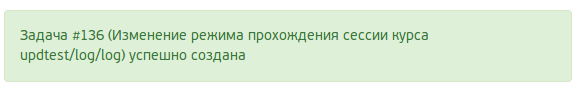
\includegraphics[height=1.5cm]{student_change_mode_task}}
	\caption{Сообщение о создании фоновой задачи}
	\label{img:student:student_change_mode_task}
\end{figure}
Для просмотра результатов выполнения задачи необходимо перейти в раздел \quotes{Фоновые задачи}, 
рассмотренный в п.~\ref{sec:mass_async_task}.


\subsection{Зачисление студентов на сессию курса списком}
Внешний вид формы зачисления студентов на сессию курса списком представлен на рис.~\ref{img:student:mass_enroll}.

\begin{figure}[H]
	\center{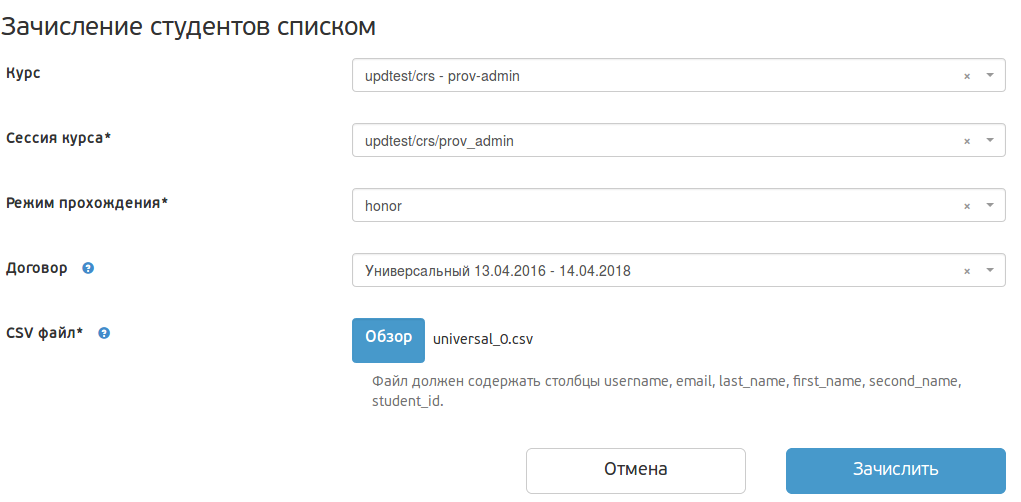
\includegraphics[width=1\linewidth]{mass_enroll}}
	\caption{Зачисление студентов на сессию курса списком}
	\label{img:student:mass_enroll}
\end{figure}

Для зачисления студентов списком необходимо:
\begin{enumerate}
	\item в выпадающем списке с автодополнением выбрать курс, который будут проходить студенты 
	(описание виджета см. в подразделе~\ref{widget:autocomplete});
	\item в выпадающем списке с автодополнением выбрать конкретную сессию этого курса 
	(описание виджета см. в подразделе~\ref{widget:autocomplete});
	\item в выпадающем списке с автодополнением выбрать один из режимов прохождения, доступных в рамках выбранной сессии 
	(описание виджета см. в подразделе~\ref{widget:autocomplete});
	\item опционально можно в выпадающем списке с автодополнением выбрать договор с вузом"=потребителем, 
	по которому осуществляется зачисление студентов (описание виджета см. в подразделе~\ref{widget:autocomplete});
	\item выбрать CSV"=файл с информацией о студентах. 
\end{enumerate}

Изначально поле \quotes{Договор} неактивно, оно активируется только после выбора сессии курса.
После выбора курса в выпадающем списке сессий будут перечислены только сессии выбранного курса, 
а в списке договоров "--- только договоры, заключенные для этого курса, либо договоры без курсов.

Для заполнения информации о студентах необходимо нажать на кнопку \quotes{Обзор} и в появившемся диалоге выбрать CSV"=файл в универсальном формате, описанном в п.~\ref{sec:csv_format}. 
После заполнения всех необходимых полей необходимо нажать на кнопку \quotes{Зачислить}.

При зачислении студентов списком для каждого выбранного студента осуществляются проверки:
\begin{itemize}
	\item студент зарегистрирован на Платформе;
	\item все данные о студенте из CSV совпадают с данными в профиле студента;
	\item студент не зачислен на выбранную сессию;
	\item если новый режим прохождения \quotes{verified} (с подтверждением личности), поле \quotes{Договор} 
	становится обязательным для заполнения; 
	\item если заполнено поле \quotes{Договор}, студент должен быть связан с вузом-потребителем из этого договора.
\end{itemize}

При загрузке файла без записей отобразится ошибка (см. рис.~\ref{img:student:mass_enroll_empty_csv}).
\begin{figure}[H]
	\center{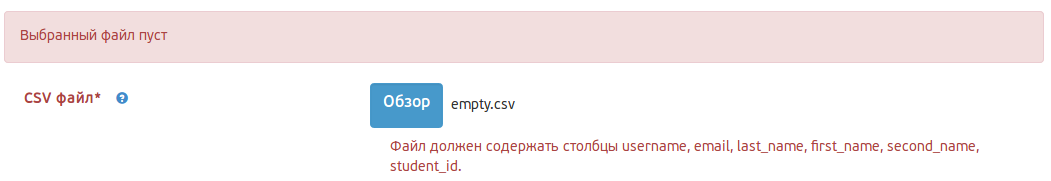
\includegraphics[width=1\linewidth]{mass_enroll_empty_csv}}
	\caption{Пустой CSV файл}
	\label{img:student:mass_enroll_empty_csv}
\end{figure}

При загрузке корректного файла создается фоновая задача для его обработки и появляется соответствующее сообщение 
(см. рис.~\ref{img:student:mass_student_enroll_task}), а также осуществляется переход на список студентов, обучающихся на курсах данного вуза.

\begin{figure}[H]
	\center{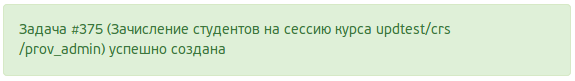
\includegraphics[height=1.5cm]{student_enroll_task}}
	\caption{Сообщение о создании фоновой задачи}
	\label{img:student:mass_student_enroll_task}
\end{figure}

Для просмотра результатов выполнения задачи необходимо перейти в раздел \quotes{Фоновые задачи}, 
рассмотренный в п.~\ref{sec:mass_async_task}.

\subsection{Изменение режима прохождения списком}
Внешний вид формы изменения режима прохождения списком представлен на рис.~\ref{img:student:mass_change_mode}.
\begin{figure}[H]
	\center{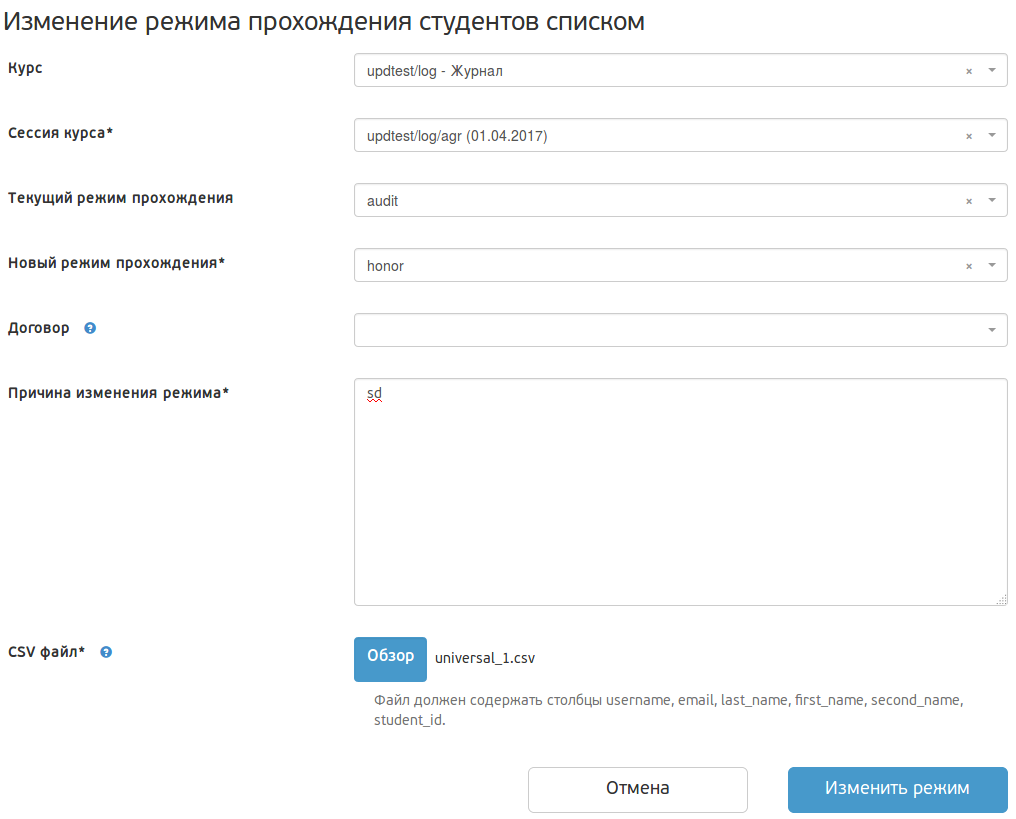
\includegraphics[width=1\linewidth]{mass_change_mode}}
	\caption{Изменение режима прохождения списком}
	\label{img:student:mass_change_mode}
\end{figure}

Для изменения режима прохождения списком необходимо:
\begin{enumerate}
	\item в выпадающем списке с автодополнением выбрать курс, на который зачислены студенты 
	(описание виджета см. в подразделе~\ref{widget:autocomplete});
	\item в выпадающем списке с автодополнением выбрать конкретную сессию этого курса 
	(описание виджета см. в подразделе~\ref{widget:autocomplete});
	\item опционально можно в выпадающем списке с автодополнением выбрать текущий режим прохождения среди 
	доступных в рамках выбранной сессии (описание виджета см. в подразделе~\ref{widget:autocomplete});
	\item в выпадающем списке с автодополнением выбрать новый режим прохождения среди доступных в рамках выбранной 
	сессии, за исключением выбранного текущего режима (описание виджета см. в подразделе~\ref{widget:autocomplete});
	\item опционально можно в выпадающем списке с автодополнением выбрать договор с вузом"=потребителем, 
	по которому осуществляется зачисление студентов (описание виджета см. в подразделе~\ref{widget:autocomplete});
	\item выбрать CSV"=файл с информацией о студентах. 
\end{enumerate}

Изначально поле \quotes{Договор} неактивно, оно активируется только после выбора сессии курса.
После выбора курса в выпадающем списке сессий будут перечислены только сессии выбранного курса, 
а в списке договоров "--- только договоры, заключенные для этого курса, либо договоры без курсов.

Для заполнения информации о студентах необходимо нажать на кнопку \quotes{Обзор} и в появившемся диалоге выбрать 
CSV"=файл в универсальном формате, описанном в п.~\ref{sec:csv_format}. 
После заполнения всех необходимых полей необходимо нажать на кнопку \quotes{Изменить режим}.

При изменении режима прохождения списком для каждого выбранного студента осуществляются проверки:
\begin{itemize}
	\item студент зарегистрирован на Платформе;
	\item все данные о студенте из CSV совпадают с данными в профиле студента;
	\item если новый режим прохождения \quotes{verified} (с подтверждением личности), поле \quotes{Договор} 
	становится обязательным для заполнения;
	\item студент был ранее зачислен на выбранную сессию;
	\item текущий режим прохождения студентом сессии отличается от выбранного нового режима прохождения.
\end{itemize}

При загрузке файла без записей отобразится ошибка (см. рис.~\ref{img:student:mass_change_mode_empty_csv}).
\begin{figure}[H]
	\center{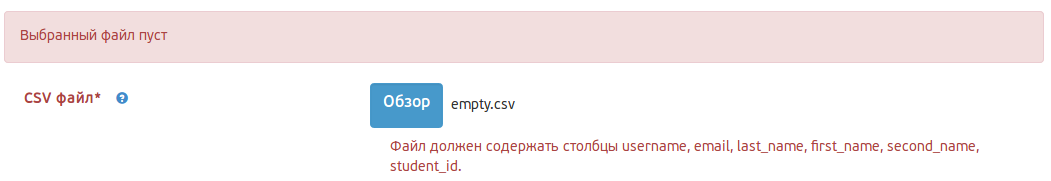
\includegraphics[width=1\linewidth]{mass_enroll_empty_csv}}
	\caption{Пустой CSV файл}
	\label{img:student:mass_change_mode_empty_csv}
\end{figure}

При загрузке корректного файла создается фоновая задача для его обработки и появляется соответствующее сообщение 
(см. рис.~\ref{img:student:mass_change_mode_task}), а также осуществляется переход на список студентов, 
обучающихся на курсах данного вуза.

\begin{figure}[H]
	\center{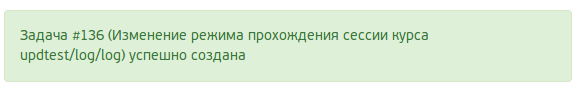
\includegraphics[height=1.5cm]{student_change_mode_task}}
	\caption{Сообщение о создании фоновой задачи}
	\label{img:student:mass_change_mode_task}
\end{figure}
Для просмотра результатов выполнения задачи необходимо перейти в раздел \quotes{Фоновые задачи}, 
рассмотренный в п.~\ref{sec:mass_async_task}.

\subsection{Заявки на привязку студентов к вузу}
Заявки на привязку студентов к вузу "--- это табличное представление, отображающее заявки 
на привязку студентов к данному вузу. Любой пользователь Платформы может подать заявку на привязку к вузу на 
странице редактирования профиля. После этого заявка появляется в списке для рассмотрения сотрудниками вуза.
Внешний вид списка представлен на рис.~\ref{img:student:bind_request_list}. 
\begin{figure}[H]
	\center{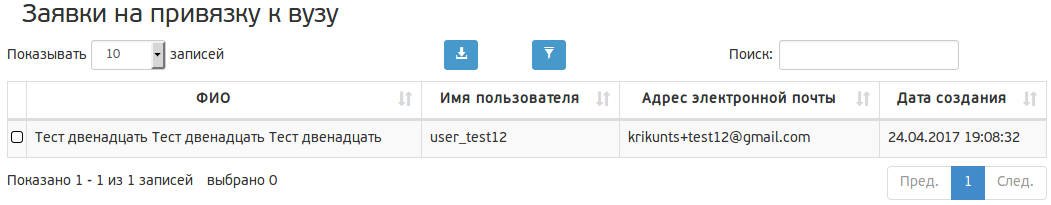
\includegraphics[width=1\linewidth]{bind_request_list}}
	\caption{Заявки на привязку студентов к вузу}
	\label{img:student:bind_request_list}
\end{figure}

Общие элементы управления табличными представления описаны в подразделе~\ref{sec:datatables}. 
Для принятия или отклонения одной или нескольких заявок нужно предварительно выбрать их, кликнув по крайнему 
левому столбцу. При выборе хотя бы одной заявки она выделяется цветом, а также активируются кнопки для принятия и 
отклонения заявок, представленные на рис.~\ref{img:student:bind_request_list_review}.
\begin{figure}[H]
	\center{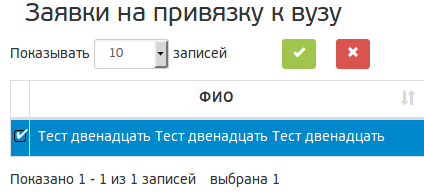
\includegraphics[height=3cm]{bind_request_list_review}}
	\caption{Кнопки принятия и отклонения заявок}
	\label{img:student:bind_request_list_review}
\end{figure}

После рассмотрения заявки (принятии или отклонении) она исчезает из списка заявок. 
Если заявка принята, указанный в заявке студент появляется в списке студентов данного вуза, 
а если отклонена - она исчезает также из списка заявок в профиле студента. 
После отклонения заявки студент может заново подать её на странице редактирования профиля.

\subsection{Студенты вуза}

Список студентов вуза "--- это табличное представление всех студентов, ассоциированных с данным вузом.
Внешний вид списка представлен на рис.~\ref{img:student:univ_student_list}. 
Элементы управления табличными представления описаны в подразделе~\ref{sec:datatables}.
Таблица содержит следующие столбцы:
\begin{itemize}
	\item ФИО студента;
	\item адрес электронной почты студента;
	\item все сессии курсов, на которые зачислен студент;
\end{itemize}

\begin{figure}[H]
	\center{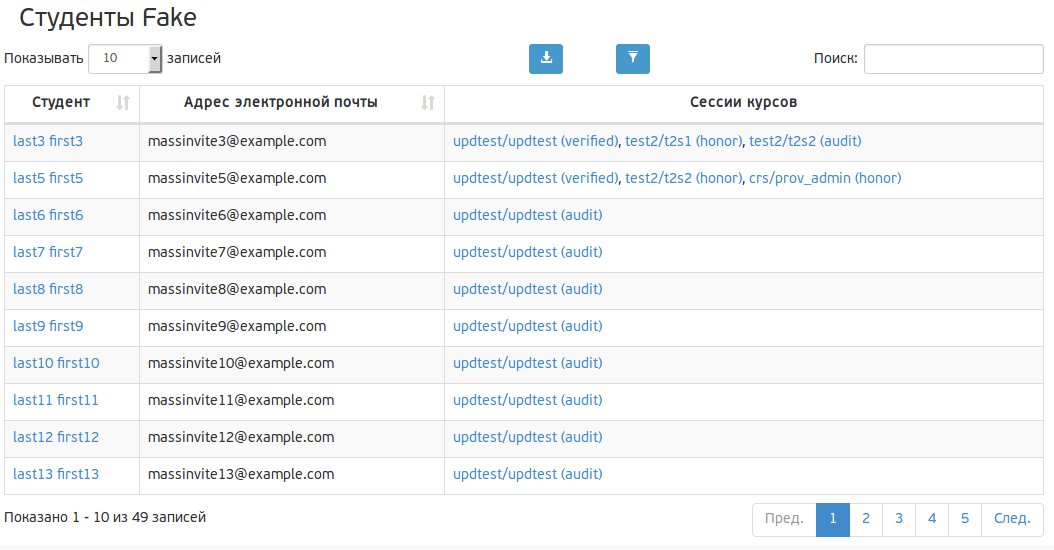
\includegraphics[width=1\linewidth]{univ_student_list}}
	\caption{Список студентов вуза}
	\label{img:student:univ_student_list}
\end{figure}

Внешний вид диалога фильтрации списка студентов представлен на рис.~\ref{img:student:univ_student_list_filter}.
Можно фильтровать список по следующим полям:
\begin{itemize}
	\item ФИО студента "--- текстовое поле;
	\item курс, на сессию которого он зачислен "--- виджет выпадающего списка с автодополнением 
	с возможностью множественного выбора (описание виджета см. в подразделе~\ref{widget:autocomplete_with_multiselect}).
\end{itemize}

 
\begin{figure}[H]
	\center{\includegraphics[height=5.5cm]{enrolled_list_filter}}
	\caption{Диалог фильтрации списка студентов вуза}
	\label{img:student:univ_student_list_filter}
\end{figure}

Каждая сессия курса в списке является ссылкой на страницу курса на сайте. 
ФИО студента является ссылкой на просмотр подробной информации о нем, 
описанной в подразделе~\ref{sec:student_detail}.

\subsection{Подробная информация о студенте вуза} \label{sec:student_detail}
Внешний вид страницы с подробной информацией представлен на рис.~\ref{img:student:student_detail}.

\begin{figure}[H]
	\center{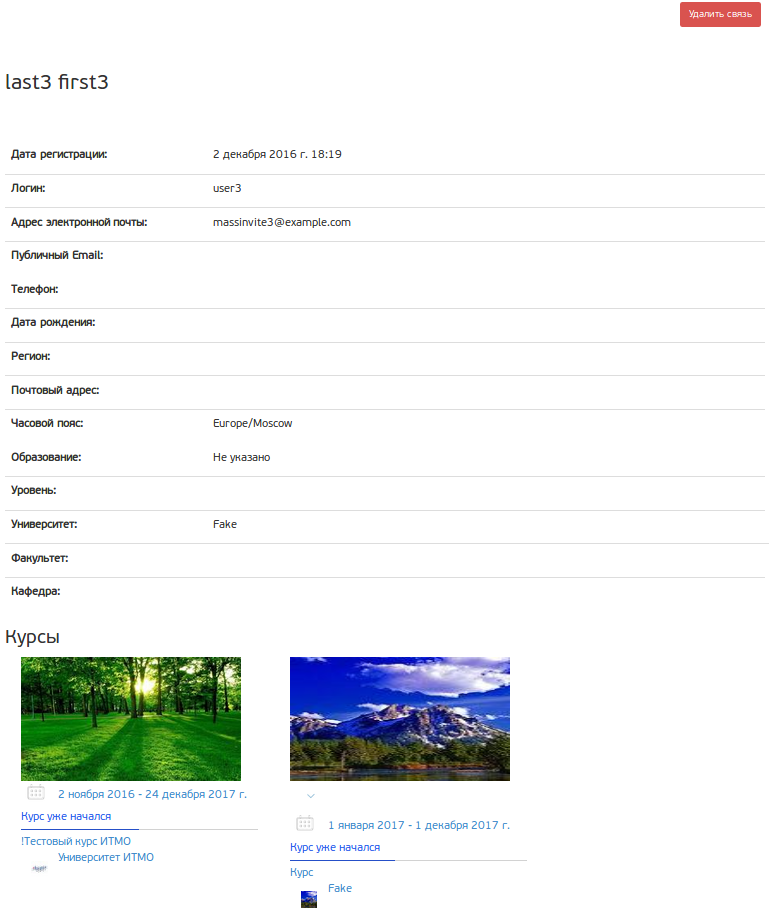
\includegraphics[width=1\linewidth]{student_detail}}
	\caption{Подробная информация о студенте}
	\label{img:student:student_detail}
\end{figure}

Для просмотра доступны следующие поля:
\begin{itemize}
	\item дата регистрации;
	\item логин;
	\item адрес электронной почты;
	\item публичный e"=mail;
	\item телефон;
	\item дата рождения;
	\item регион;
	\item почтовый адрес;
	\item часовой пояс;
	\item образование;
	\item степень;
	\item университет;
	\item факультет;
	\item кафедра;
	\item список сессий курсов, на которые записан студент.
\end{itemize}

Администратор вуза может разорвать связь студента с данным вузом, нажав на кнопку \quotes{Удалить связь}. 
При нажатии на эту кнопку отображается диалог подтверждения, представленный на рис.~\ref{img:student:unbind_dialog}.

\begin{figure}[H]
	\center{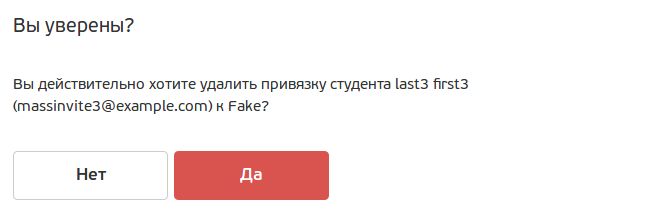
\includegraphics[width=1\linewidth]{unbind_dialog}}
	\caption{Диалог подтверждения}
	\label{img:student:unbind_dialog}
\end{figure}
После подтверждения происходит переход на список студентов вуза, в котором данный студент больше не отображается.


\subsection{Заявки на зачисление}

Заявки на зачисление "--- это табличное представление заявок на зачисление студентов, 
поданных данным вузом в качестве вуза"=потребителя. 
Элементы управления табличными представления описаны в подразделе~\ref{sec:datatables}.
Внешний вид списка представлен на рис.~\ref{img:student:enroll_req_list}. 

\begin{figure}[H]
	\center{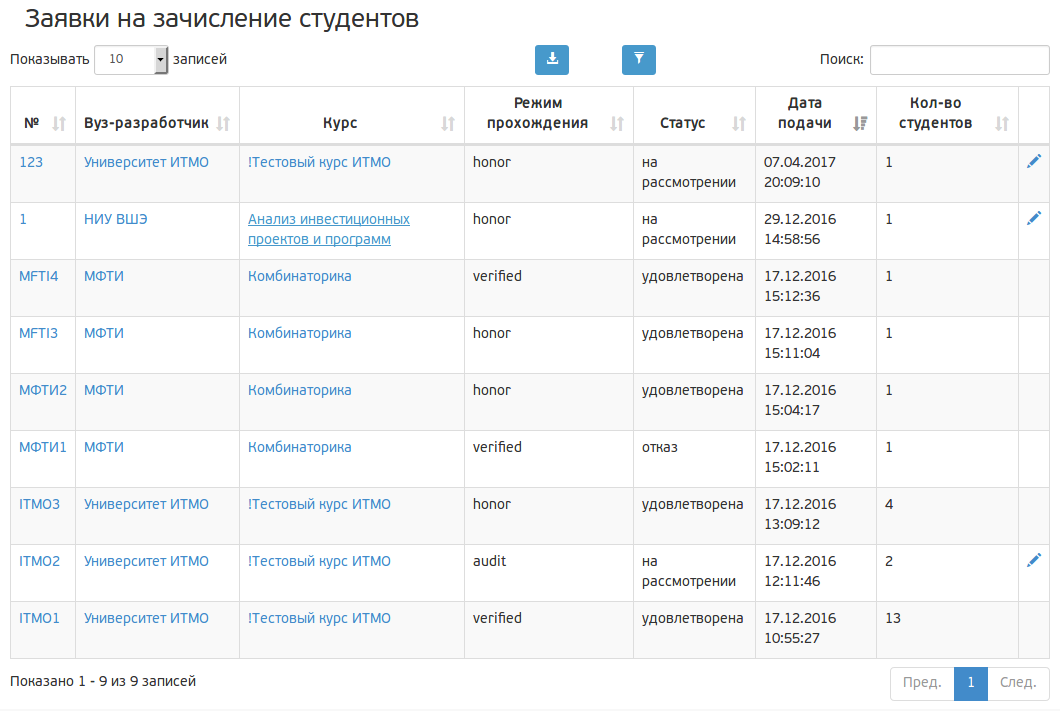
\includegraphics[width=1\linewidth]{enroll_req_list}}
	\caption{Список заявок на зачисление}
	\label{img:student:enroll_req_list}
\end{figure}

Таблица содержит следующие столбцы:
\begin{itemize}
	\item номер заявки;
	\item вуз"=разработчик;
	\item курс;
	\item режим прохождения;
	\item статус;
	\item дата подачи;
	\item количество студентов в заявке.
\end{itemize}

Крайний правый столбец содержит ссылку на редактирование заявки, если она находится в состоянии \quotes{на рассмотрении}.

Внешний вид диалога фильтрации списка заявок представлен на рис.~\ref{img:student:enroll_req_list_filter}.
Можно фильтровать список по следующим параметрам:
\begin{itemize}
	\item вуз"=разработчик "--- виджет выпадающего списка с автодополнением с возможностью множественного выбора 
	(описание виджета см. в подразделе~\ref{widget:autocomplete_with_multiselect});
	\item курс "--- виджет выпадающего списка с автодополнением с возможностью множественного выбора 
	(описание виджета см. в подразделе~\ref{widget:autocomplete_with_multiselect});
	\item режим прохождения "--- виджет выпадающего списка с автодополнением с возможностью множественного выбора 
	(описание виджета см. в подразделе~\ref{widget:autocomplete_with_multiselect});
	\item статус "--- виджет выпадающего списка с автодополнением с возможностью множественного выбора 
	(описание виджета см. в подразделе~\ref{widget:autocomplete_with_multiselect});
	\item диапазон дат подачи "--- виджеты выбора даты и времени 
	(описание виджета см. в подразделе~\ref{widget:date_time_picker});
	\item диапазон количества студентов в заявке "--- числовое поле.
\end{itemize}

\begin{figure}[H]
	\center{\includegraphics[height=9.1cm]{enroll_req_list_filter}}
	\caption{Диалог фильтрации списка заявок на зачисление}
	\label{img:student:enroll_req_list_filter}
\end{figure}
Номер заявки в таблице является ссылкой на страницу просмотра подробной информации о заявке, 
описанной в подразделе~\ref{sec:enroll_req_detail}.

\subsection{Подробная информация о заявке на зачисление} \label{sec:enroll_req_detail}
Внешний вид страницы с подробной информацией о заявке на зачисление представлен на рис.~\ref{img:student:enroll_req_detail}.
\begin{figure}[H]
	\center{\includegraphics[height=9.1cm]{enroll_req_detail}}
	\caption{Подробная информация о заявке на зачисление}
	\label{img:student:enroll_req_detail}
\end{figure}

Для просмотра доступны следующие поля:
\begin{itemize}
	\item номер заявки;
	\item статус;
	\item причина отклонения (если есть);
	\item вуз"=потребитель;
	\item курс;
	\item сессия курса;
	\item режим прохождения;
	\item договор с вузом"=разработчиком;
	\item количество студентов в заявке;
	\item дата подачи заявки;
	\item список студентов;
\end{itemize}

Если на страницу заявки заходит администратор вуза, который указан в ней в качестве потребителя, ему доступны 
следующие действия:
\begin{itemize}
	\item если заявка находится в состоянии \quotes{на рассмотрении}, появляется кнопка перехода в режим 
	редактирования заявки. \vcenteredinclude[height=20px]{edit}
	\item появляется кнопка удаления заявки \vcenteredinclude[height=20px]{delete}.
\end{itemize}

Если заявка находится в статусе \quotes{на рассмотрении}, при нажатии кнопки удаления отображается диалог подтверждения, 
представленный на рис.~\ref{img:student:req_delete_confirm} 
\begin{figure}[H]
	\center{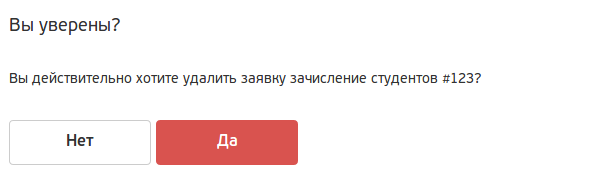
\includegraphics[height=3.5cm]{req_delete_confirm}}
	\caption{Диалог подтверждения удаления заявки}
	\label{img:student:req_delete_confirm}
\end{figure}
При подтверждении происходит удаление заявки и осуществляется переход на страницу со списком заявок на зачисление.

Если заявка находится в другом статусе, то при нажатии кнопки удаления появляется сообщение о невозможности удаления 
заявки с указанием причины (см. рис~\ref{img:student:req_cannot_delete})
\begin{figure}[H]
	\center{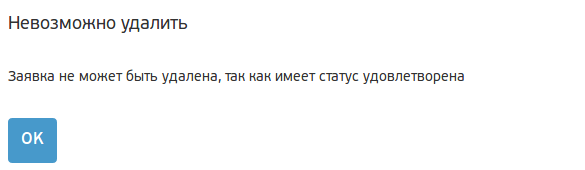
\includegraphics[height=3.5cm]{req_cannot_delete}}
	\caption{Сообщение о невозможности удаления заявки}
	\label{img:student:req_cannot_delete}
\end{figure}

Если на страницу заявки в состоянии \quotes{на рассмотрении} заходит администратор вуза, 
указанного в ней в качестве поставщика, для него доступны кнопки \quotes{Принять заявку} и 
\quotes{Отклонить заявку}, представленные на рис.~\ref{img:student:req_detail_buttons}.
\begin{figure}[H]
	\center{\includegraphics[height=1cm]{req_detail_buttons}}
	\caption{Кнопки смены состояния заявки}
	\label{img:student:req_detail_buttons}
\end{figure}

При нажатии на кнопку \quotes{Принять заявку} студенты из заявки зачисляются на указанную в ней сессию курса 
с указанным режимом прохождения, для этого создается фоновая задача и отображается соответствующее сообщение 
(см. рис.~\ref{img:student:req_accept}), а статус заявки изменяется на \quotes{в обработке}.
\begin{figure}[H]
	\center{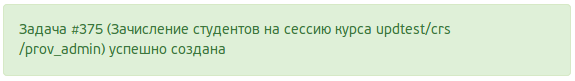
\includegraphics[height=1.5cm]{student_enroll_task}}
	\caption{Сообщение о создании фоновой задачи}
	\label{img:student:req_accept}
\end{figure}

Существует несколько причин, по которым принять заявку нельзя и кнопка \quotes{Принять заявку} не показывается:
\begin{itemize}
	\item невозможно зачислить студентов на завершенную сессию курса;
	\item количество студентов в заявке превышает свободное количество студентов по договору.
\end{itemize}

При нажатии на кнопку \quotes{Отклонить заявку} появляется диалог для указания причины отказа, 
представленный на рис.~\ref{img:student:req_detail_decline}
\begin{figure}[H]
	\center{\includegraphics[height=4cm]{req_detail_decline}}
	\caption{Диалог указания причины отказа}
	\label{img:student:req_detail_decline}
\end{figure}
Для того, чтобы отклонить заявку нужно ввести причину отклонения заявки в текстовое поле диалога 
и нажать кнопку \quotes{Отклонить заявку} внизу диалога. После этого статус заявки изменяется на \quotes{отказ}.


\subsection{Заявки на изменение режима прохождения сессии курса}

Заявки на изменение режима прохождения сессии курса "--- это табличное представление заявок на изменение 
режима прохождения сессии курса, поданных данным вузом в качестве вуза"=потребителя. 
Элементы управления табличными представления описаны в подразделе~\ref{sec:datatables}.
Внешний вид списка представлен на рис.~\ref{img:student:change_mode_req_list}. 

\begin{figure}[H]
	\center{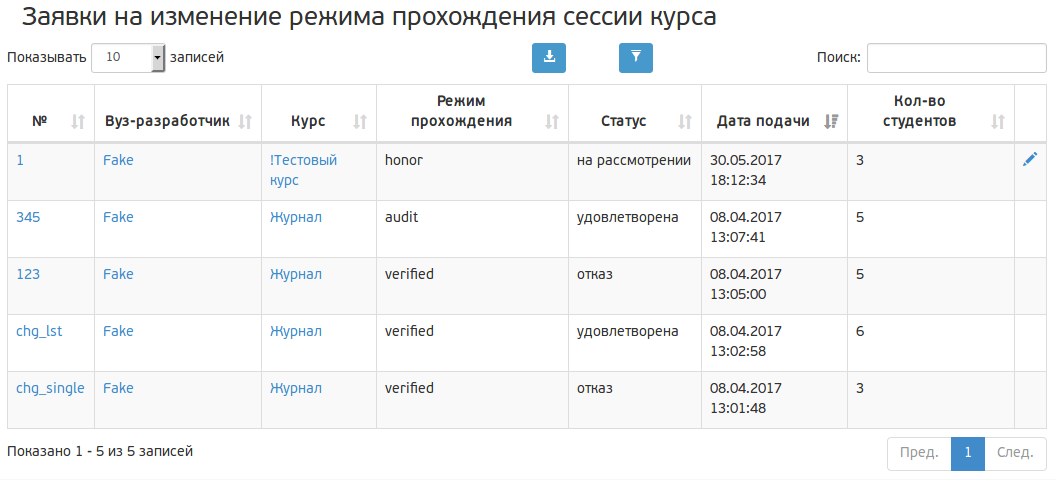
\includegraphics[width=1\linewidth]{change_mode_req_list}}
	\caption{Список заявок на изменение режима прохождения сессии курса}
	\label{img:student:change_mode_req_list}
\end{figure}

Таблица содержит следующие столбцы:
\begin{itemize}
	\item номер заявки;
	\item вуз"=разработчик;
	\item курс;
	\item режим прохождения;
	\item статус;
	\item дата подачи;
	\item количество студентов в заявке.
\end{itemize}
Крайний правый столбец содержит ссылку на редактирование заявки, если она находится в состоянии \quotes{на рассмотрении}.


Внешний вид диалога фильтрации списка заявок представлен на рис.~\ref{img:student:change_mode_req_list_filter}.
\begin{figure}[H]
	\center{\includegraphics[height=9.1cm]{enroll_req_list_filter}}
	\caption{Диалог фильтрации списка заявок на изменение режима прохождения сессии курса}
	\label{img:student:change_mode_req_list_filter}
\end{figure}

Можно фильтровать список по следующим параметрам:
\begin{itemize}
	\item вуз"=разработчик "--- виджет выпадающего списка с автодополнением с возможностью множественного выбора 
	(см. подраздел~\ref{widget:autocomplete_with_multiselect});
	\item курс "--- виджет выпадающего списка с автодополнением с возможностью множественного выбора 
	(см. подраздел~\ref{widget:autocomplete_with_multiselect});
	\item режим прохождения "--- виджет выпадающего списка с автодополнением с возможностью множественного выбора 
	(см. подраздел~\ref{widget:autocomplete_with_multiselect});
	\item статус "--- виджет выпадающего списка с автодополнением с возможностью множественного выбора 
	(см. подраздел~\ref{widget:autocomplete_with_multiselect});
	\item диапазон дат подачи "--- виджеты выбора даты и времени 
	(см. подраздел~\ref{widget:date_time_picker});
	\item диапазон количества студентов в заявке "--- числовое поле.
\end{itemize}

Номер заявки в таблице является ссылкой на страницу просмотра подробной информации о заявке, 
описанной в подразделе~\ref{sec:change_mode_req_detail}.

\subsection{Подробная информация о заявке на изменение режима прохождения сессии курса} 
\label{sec:change_mode_req_detail}

Внешний вид страницы с подробной информацией о заявке на изменение режима прохождения сессии курса представлен 
на рис.~\ref{img:student:change_mode_req_detail}.
\begin{figure}[H]
	\center{\includegraphics[height=9.1cm]{change_mode_req_detail}}
	\caption{Подробная информация о заявке на изменение режима прохождения сессии курса}
	\label{img:student:change_mode_req_detail}
\end{figure}

Для просмотра доступны следующие поля:
\begin{itemize}
	\item номер заявки;
	\item статус;
	\item причина отклонения (если есть);
	\item вуз"=потребитель;
	\item курс;
	\item сессия курса;
	\item режим прохождения;
	\item договор с вузом"=разработчиком;
	\item количество студентов в заявке;
	\item дата подачи заявки;
	\item список студентов.
\end{itemize}

Если на страницу заявки заходит администратор вуза, который указан в ней в качестве потребителя, ему доступны 
следующие действия:
\begin{itemize}
	\item если заявка находится в состоянии \quotes{на рассмотрении}, появляется кнопка перехода в режим редактирования 
	заявки. \vcenteredinclude[height=20px]{edit}
	\item появляется кнопка удаления заявки \vcenteredinclude[height=20px]{delete}.
\end{itemize}

Если заявка находится в статусе \quotes{на рассмотрении}, при нажатии кнопки удаления отображается диалог подтверждения, 
представленный на рис.~\ref{img:student:req_change_mode_delete_confirm} 
\begin{figure}[H]
	\center{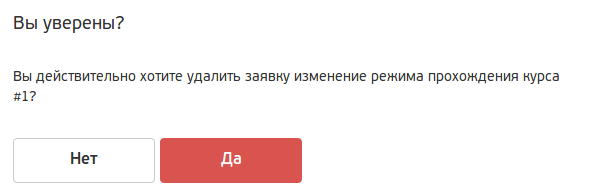
\includegraphics[height=3.5cm]{req_change_mode_delete_confirm}}
	\caption{Диалог подтверждения удаления заявки}
	\label{img:student:req_change_mode_delete_confirm}
\end{figure}
При подтверждении происходит удаление заявки и осуществляется переход на страницу со списком заявок на изменение 
режима прохождения.

Если заявка находится в другом статусе, то при нажатии кнопки удаления появляется сообщение о невозможности удаления 
заявки с указанием причины (см. рис~\ref{img:student:req_change_mode_cannot_delete})
\begin{figure}[H]
	\center{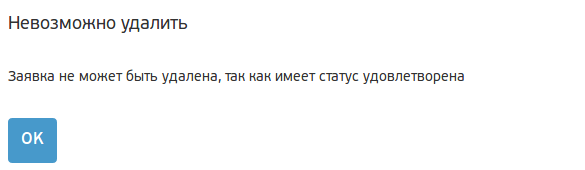
\includegraphics[height=3.5cm]{req_cannot_delete}}
	\caption{Сообщение о невозможности удаления заявки}
	\label{img:student:req_change_mode_cannot_delete}
\end{figure}

Если на страницу заявки в состоянии \quotes{на рассмотрении} заходит администратор вуза, 
указанного в ней в качестве поставщика, для него доступны кнопки \quotes{Принять заявку} и 
\quotes{Отклонить заявку}, представленные на рис.~\ref{img:student:change_mode_req_detail_buttons}.

\begin{figure}[H]
	\center{\includegraphics[height=1cm]{req_detail_buttons}}
	\caption{Кнопки смены состояния заявки}
	\label{img:student:change_mode_req_detail_buttons}
\end{figure}

При нажатии на кнопку \quotes{Принять заявку} для студентов из заявки изменяется режим прохождения указанной  
сессии курса, для этого создается фоновая задача и отображается соответствующее сообщение 
(см. рис.~\ref{img:student:req_change_mode_accept}), а статус заявки изменяется на \quotes{в обработке}.
\begin{figure}[H]
	\center{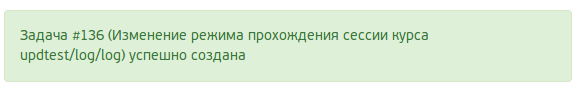
\includegraphics[height=1.5cm]{student_change_mode_task}}
	\caption{Сообщение о создании фоновой задачи}
	\label{img:student:req_change_mode_accept}
\end{figure}

При нажатии на кнопку \quotes{Отклонить заявку} появляется диалог для указания причины отказа, 
представленный на рис.~\ref{img:student:change_mode_req_detail_decline}
\begin{figure}[H]
	\center{\includegraphics[height=4cm]{req_detail_decline}}
	\caption{Диалог указания причины отказа}
	\label{img:student:change_mode_req_detail_decline}
\end{figure}
Для того, чтобы отклонить заявку нужно ввести причину отклонения заявки в текстовое поле диалога 
и нажать кнопку \quotes{Отклонить заявку} внизу диалога. После этого статус заявки изменяется на \quotes{отказ}.


\subsection{Создание заявки на зачисление}
Внешний вид формы создания заявки на зачисления студентов представлен на рис.~\ref{img:student:enroll_req_create}.

\begin{figure}[H]
	\center{\includegraphics[width=1\linewidth]{enroll_req_create}}
	\caption{Создание заявки на зачисление студентов}
	\label{img:student:enroll_req_create}
\end{figure}

Для создания заявки на зачисление студентов необходимо:
\begin{enumerate}
	\item задать номер заявки в текстовом поле;
	\item в выпадающем списке с автодополнением выбрать вуз"=поставщик курса
	(описание виджета см. в подразделе~\ref{widget:autocomplete});
	\item в выпадающем списке с автодополнением выбрать курс выбранного вуза, который будут проходить студенты 
	(описание виджета см. в подразделе~\ref{widget:autocomplete});
	\item в выпадающем списке с автодополнением выбрать конкретную сессию этого курса 
	(описание виджета см. в подразделе~\ref{widget:autocomplete});
	\item в выпадающем списке с автодополнением выбрать один из режимов прохождения, доступных в рамках выбранной сессии 
	(описание виджета см. в подразделе~\ref{widget:autocomplete});
	\item опционально можно в выпадающем списке с автодополнением выбрать договор с выбранным вузом"=поставщиком, 
	по которому осуществляется зачисление студентов (описание виджета см. в подразделе~\ref{widget:autocomplete});
	\item выбрать одного или нескольких студентов из числа уже зарегистрированных на Платформе студентов данного вуза 
	при помощи виджета выпадающего списка с автодополнением с возможностью множественного выбора 
	(описание виджета см. в подразделе~\ref{widget:autocomplete_with_multiselect}). 
\end{enumerate}


Изначально поля \quotes{Договор} и \quotes{Студенты} неактивны, они активируются только после выбора сессии курса.
После выбора вуза"=поставщика в выпадающем списке курсов будут перечислены только курсы, предоставляемые этим вузом.
После выбора курса в выпадающем списке сессий будут перечислены только сессии выбранного курса, 
а в списке договоров "--- только договоры, заключенные данным вузом с вузом"=разработчиком для этого курса, 
либо договоры без курсов.
После выбора сессии курса в списке студентов будут перечислены только те студенты данного вуза,
которые еще не зачислены на выбранную сессию курса.
В случае выбора режима \quotes{verified} (с подтверждением личности), поле \quotes{Договор} становится 
обязательным для заполнения. 

В случае, если заполнено поле \quotes{Договор} и количество свободных мест по договору меньше, 
чем количество выбранных для зачисления студентов, система выдаст предупреждение 
(рис.~\ref{img:student:enroll_req_create_student_error}), но на возможность зачисления студентов оно не влияет.

\begin{figure}[H]
	\center{\includegraphics[width=1\linewidth]{enroll_student_error}}
	\caption{Превышение количества студентов по договору.}
	\label{img:student:enroll_req_create_student_error}
\end{figure}

После заполнения всех полей необходимо нажать на кнопку \quotes{Создать}.

При создании заявки на зачисление осуществляется проверка возможных дубликатов среди других заявок на зачисление, 
находящихся в статусе \quotes{на рассмотрении}. Проверяется полное совпадение всех полей, кроме номера заявки. 
В случае, если среди существующих заявок находится дубликат создаваемой заявки, выводится соответствующее сообщение 
(см. рис.~\ref{img:student:req_enroll_duplicate_msg}) со ссылкой на найденную заявку-дубликат, 
а новая заявка не создается.

\begin{figure}[H]
	\center{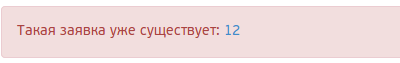
\includegraphics[height=1.1cm]{req_duplicate_msg}}
	\caption{Сообщение о найденном дубликате}
	\label{img:student:req_enroll_duplicate_msg}
\end{figure}

\subsection{Создание заявки на зачисление списком}
Внешний вид формы создания заявки на зачисления студентов списком представлен 
на рис.~\ref{img:student:mass_enroll_req_create}.

\begin{figure}[H]
	\center{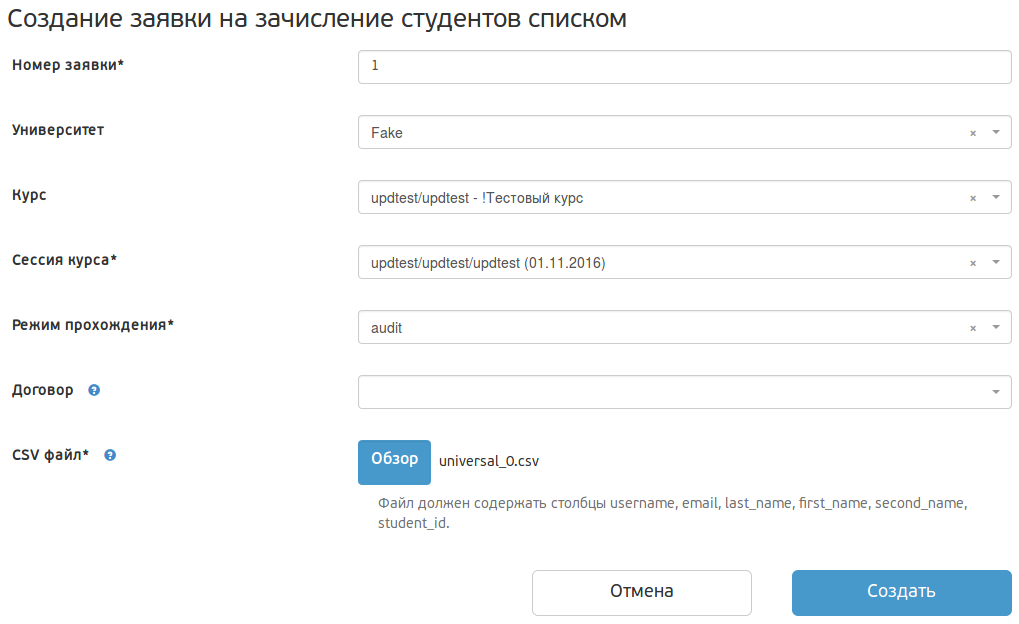
\includegraphics[width=1\linewidth]{mass_enroll_req_create}}
	\caption{Создание заявки на зачисление студентов списком}
	\label{img:student:mass_enroll_req_create}
\end{figure}

Для создания заявки на зачисление студентов списком необходимо:
\begin{enumerate}
	\item задать номер заявки в текстовом поле;
	\item в выпадающем списке с автодополнением выбрать вуз"=поставщик курса
	(описание виджета см. в подразделе~\ref{widget:autocomplete});
	\item в выпадающем списке с автодополнением выбрать курс выбранного вуза, который будут проходить студенты 
	(описание виджета см. в подразделе~\ref{widget:autocomplete});
	\item в выпадающем списке с автодополнением выбрать конкретную сессию этого курса 
	(описание виджета см. в подразделе~\ref{widget:autocomplete});
	\item в выпадающем списке с автодополнением выбрать один из режимов прохождения, доступных в рамках выбранной сессии 
	(описание виджета см. в подразделе~\ref{widget:autocomplete});
	\item опционально можно в выпадающем списке с автодополнением выбрать договор с выбранным вузом"=поставщиком, 
	по которому осуществляется зачисление студентов (описание виджета см. в подразделе~\ref{widget:autocomplete});
	\item выбрать CSV"=файл с информацией о студентах. 
\end{enumerate}


Изначально поле \quotes{Договор} неактивно, оно активируется только после выбора сессии курса.
После выбора вуза"=поставщика в выпадающем списке курсов будут перечислены только курсы, предоставляемые этим вузом.
После выбора курса в выпадающем списке сессий будут перечислены только сессии выбранного курса, 
а в списке договоров "--- только договоры, заключенные данным вузом с вузом"=разработчиком для этого курса, либо договоры без курсов.
В случае выбора режима \quotes{verified} (с подтверждением личности), поле \quotes{Договор} становится обязательным 
для заполнения. 

Для заполнения информации о студентах необходимо нажать на кнопку \quotes{Обзор} и в появившемся диалоге выбрать 
CSV"=файл в универсальном формате, описанном в п.~\ref{sec:csv_format}. 
После заполнения всех необходимых полей необходимо нажать на кнопку \quotes{Создать}.

При загрузке файла без записей отобразится ошибка (см. рис.~\ref{img:student:req_mass_enroll_empty_csv}).
\begin{figure}[H]
	\center{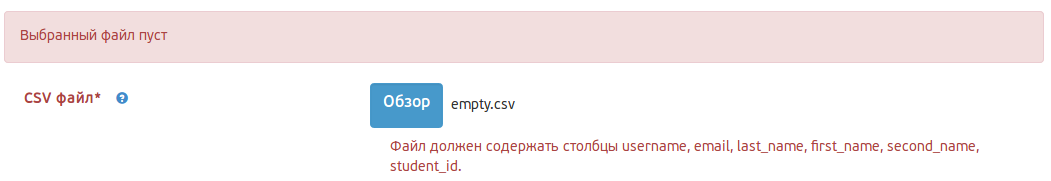
\includegraphics[width=1\linewidth]{mass_enroll_empty_csv}}
	\caption{Пустой CSV файл}
	\label{img:student:req_mass_enroll_empty_csv}
\end{figure}

При создании заявки на зачисление списком осуществляется проверка возможных дубликатов среди других заявок на зачисление,
находящихся в статусе \quotes{на рассмотрении}. Проверяется полное совпадение всех полей, кроме номера заявки. 
В случае, если среди существующих заявок находится дубликат создаваемой заявки, выводится соответствующее сообщение 
(см. рис.~\ref{img:student:req_mass_enroll_duplicate_msg}) со ссылкой на найденную заявку-дубликат, 
а новая заявка не создается.

\begin{figure}[H]
	\center{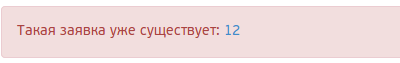
\includegraphics[height=1.1cm]{req_duplicate_msg}}
	\caption{Сообщение о найденном дубликате}
	\label{img:student:req_mass_enroll_duplicate_msg}
\end{figure}


При загрузке корректного файла создается фоновая задача для его обработки и появляется соответствующее сообщение 
(см. рис.~\ref{img:student:req_mass_enroll_task}), а также осуществляется переход на список заявок на зачисление.

\begin{figure}[H]
	\center{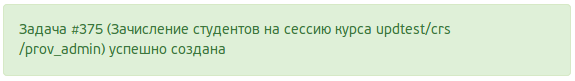
\includegraphics[height=1.5cm]{student_enroll_task}}
	\caption{Сообщение о создании фоновой задачи}
	\label{img:student:req_mass_enroll_task}
\end{figure}
Для просмотра результатов выполнения задачи необходимо перейти в раздел \quotes{Фоновые задачи}, 
рассмотренный в п.~\ref{sec:mass_async_task}.

\subsection{Создание заявки на изменение режима прохождения сессии курса студентами}

Внешний вид формы создания заявки на изменение режима прохождения сессии курса студентами
представлен на рис.~\ref{img:student:change_mode_req_create}.

\begin{figure}[H]
	\center{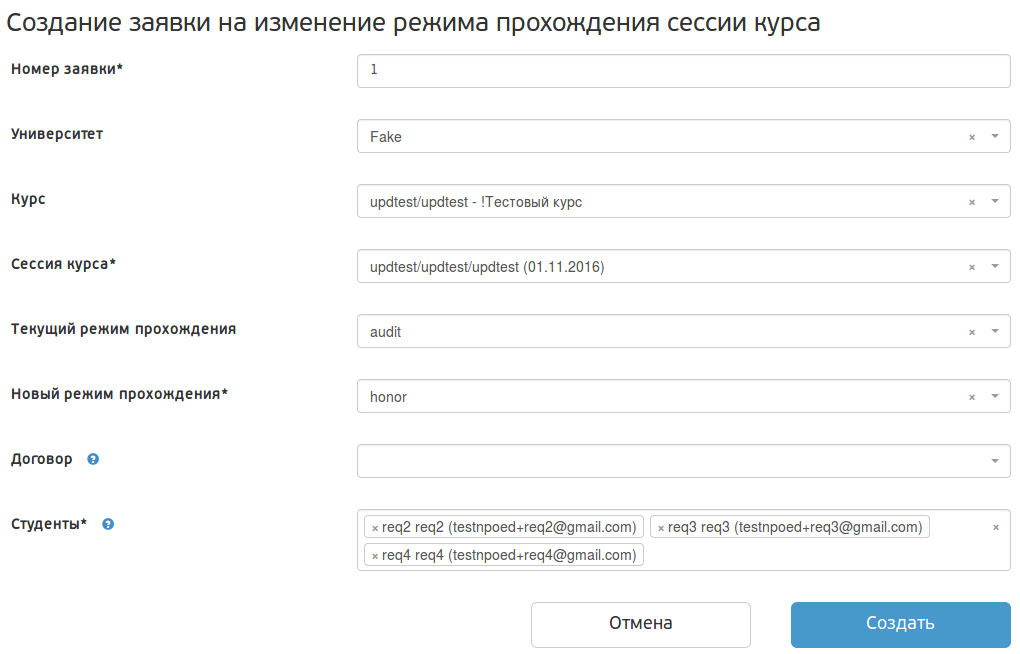
\includegraphics[width=1\linewidth]{change_mode_req_create}}
	\caption{Создание заявки на изменение режима прохождения сессии курса студентами}
	\label{img:student:change_mode_req_create}
\end{figure}

Для создания заявки на изменение режима прохождения сессии курса студентами необходимо:
\begin{enumerate}
	\item задать номер заявки в текстовом поле;
	\item в выпадающем списке с автодополнением выбрать вуз"=поставщик курса
	(описание виджета см. в подразделе~\ref{widget:autocomplete});
	\item в выпадающем списке с автодополнением выбрать курс выбранного вуза, который будут проходить студенты 
	(описание виджета см. в подразделе~\ref{widget:autocomplete});
	\item в выпадающем списке с автодополнением выбрать конкретную сессию этого курса 
	(описание виджета см. в подразделе~\ref{widget:autocomplete});
	\item опционально можно в выпадающем списке с автодополнением выбрать текущий режим прохождения среди 
	доступных в рамках выбранной сессии (описание виджета см. в подразделе~\ref{widget:autocomplete});
	\item в выпадающем списке с автодополнением выбрать новый режим прохождения среди доступных в рамках выбранной 
	сессии, за исключением выбранного текущего режима (описание виджета см. в подразделе~\ref{widget:autocomplete});
	\item опционально можно в выпадающем списке с автодополнением выбрать договор с выбранным вузом"=поставщиком, 
	по которому осуществляется зачисление студентов (описание виджета см. в подразделе~\ref{widget:autocomplete});
	\item выбрать одного или нескольких студентов из числа уже зарегистрированных на Платформе студентов данного вуза 
	при помощи виджета выпадающего списка с автодополнением с возможностью множественного выбора 
	(описание виджета см. в подразделе~\ref{widget:autocomplete_with_multiselect}). 
\end{enumerate}


Изначально поля \quotes{Договор} и \quotes{Студенты} неактивны, они активируются только после выбора сессии курса.
После выбора вуза"=поставщика в выпадающем списке курсов будут перечислены только курсы, предоставляемые этим вузом.
После выбора курса в выпадающем списке сессий будут перечислены только сессии выбранного курса, 
а в списке договоров "--- только договоры, заключенные данным вузом с вузом"=разработчиком для этого курса, 
либо договоры без курсов.
После выбора текущего режима прохождения в списке студентов будут перечислены только те студенты данного вуза, 
которые были зачислены на выбранную сессию курса с этим режимом прохождения.
После выбора нового режима прохождения в списке студентов будут перечислены только те студенты данного вуза, 
которые были зачислены на выбранную сессию курса с режимом прохождения, отличным от выбранного.
В случае установки нового режима в значение \quotes{verified} (с подтверждением личности), поле \quotes{Договор} 
становится обязательным для заполнения. 

В случае, если заполнено поле \quotes{Договор} и количество свободных мест по договору меньше, 
чем количество выбранных для зачисления студентов, система выдаст предупреждение 
(рис.~\ref{img:student:change_mode_req_create_student_error}), но на возможность зачисления студентов оно не влияет.

\begin{figure}[H]
	\center{\includegraphics[width=1\linewidth]{enroll_student_error}}
	\caption{Превышение количества студентов по договору.}
	\label{img:student:change_mode_req_create_student_error}
\end{figure}

После заполнения всех полей необходимо нажать на кнопку \quotes{Создать}.

При создании заявки на изменение режима прохождения осуществляется проверка возможных дубликатов среди других заявок 
на изменение режима прохождения, находящихся в статусе \quotes{на рассмотрении}. 
Проверяется полное совпадение всех полей, кроме номера заявки. 
В случае, если среди существующих заявок находится дубликат создаваемой заявки, выводится соответствующее сообщение 
(см. рис.~\ref{img:student:req_change_mode_duplicate_msg}) со ссылкой на найденную заявку-дубликат, 
а новая заявка не создается.

\begin{figure}[H]
	\center{\includegraphics[height=1.1cm]{req_duplicate_msg}}
	\caption{Сообщение о найденном дубликате}
	\label{img:student:req_change_mode_duplicate_msg}
\end{figure}

\subsection{Создание заявки на изменение режима прохождения сессии курса студентами списком}
Внешний вид формы создания заявки на изменение режима прохождения сессии курса студентами списком 
представлен на рис.~\ref{img:student:mass_change_mode_req_create}.

\begin{figure}[H]
	\center{\includegraphics[width=1\linewidth]{mass_change_mode_req_create}}
	\caption{Создание заявки на изменение режима прохождения сессии курса студентами списком}
	\label{img:student:mass_change_mode_req_create}
\end{figure}

Для создания заявки на изменение режима прохождения сессии курса студентами списком необходимо:
\begin{enumerate}
	\item задать номер заявки в текстовом поле;
	\item в выпадающем списке с автодополнением выбрать вуз"=поставщик курса
	(описание виджета см. в подразделе~\ref{widget:autocomplete});
	\item в выпадающем списке с автодополнением выбрать курс выбранного вуза, который будут проходить студенты 
	(описание виджета см. в подразделе~\ref{widget:autocomplete});
	\item в выпадающем списке с автодополнением выбрать конкретную сессию этого курса 
	(описание виджета см. в подразделе~\ref{widget:autocomplete});
	\item опционально можно в выпадающем списке с автодополнением выбрать текущий режим прохождения среди 
	доступных в рамках выбранной сессии (описание виджета см. в подразделе~\ref{widget:autocomplete});
	\item в выпадающем списке с автодополнением выбрать новый режим прохождения среди доступных в рамках выбранной 
	сессии, за исключением выбранного текущего режима (описание виджета см. в подразделе~\ref{widget:autocomplete});
	\item опционально можно в выпадающем списке с автодополнением выбрать договор с выбранным вузом"=поставщиком, 
	по которому осуществляется зачисление студентов (описание виджета см. в подразделе~\ref{widget:autocomplete});
	\item выбрать CSV"=файл с информацией о студентах.
\end{enumerate}

Изначально поле \quotes{Договор} неактивно, оно активируется только после выбора сессии курса.
После выбора вуза"=поставщика в выпадающем списке курсов будут перечислены только курсы, предоставляемые этим вузом.
После выбора курса в выпадающем списке сессий будут перечислены только сессии выбранного курса, 
а в списке договоров "--- только договоры, заключенные данным вузом с вузом"=разработчиком для этого курса, 
либо договоры без курсов.
После выбора текущего режима прохождения в списке студентов будут перечислены только те студенты данного вуза, 
которые были зачислены на выбранную сессию курса с этим режимом прохождения.
После выбора нового режима прохождения в списке студентов будут перечислены только те студенты данного вуза, 
которые были зачислены на выбранную сессию курса с режимом прохождения, отличным от выбранного.

В случае установки нового режима в значение \quotes{verified} (с подтверждением личности), поле \quotes{Договор} 
становится обязательным для заполнения. 


Для заполнения информации о студентах необходимо нажать на кнопку \quotes{Обзор} и в появившемся диалоге выбрать 
CSV"=файл в универсальном формате, описанном в п.~\ref{sec:csv_format}. 
После заполнения всех необходимых полей необходимо нажать на кнопку \quotes{Создать}.

При загрузке файла без записей отобразится ошибка (см. рис.~\ref{img:student:req_mass_change_mode_empty_csv}).
\begin{figure}[H]
	\center{\includegraphics[width=1\linewidth]{mass_enroll_empty_csv}}
	\caption{Пустой CSV файл}
	\label{img:student:req_mass_change_mode_empty_csv}
\end{figure}

При создании заявки на изменение режима прохождения списком осуществляется проверка возможных дубликатов среди других 
заявок на изменение режима прохождения, находящихся в статусе \quotes{на рассмотрении}. 
Проверяется полное совпадение всех полей, кроме номера заявки. 
В случае, если среди существующих заявок находится дубликат создаваемой заявки, выводится соответствующее сообщение 
(см. рис.~\ref{img:student:req_mass_change_mode_duplicate_msg}) со ссылкой на найденную заявку-дубликат, 
а новая заявка не создается.

\begin{figure}[H]
	\center{\includegraphics[height=1.1cm]{req_duplicate_msg}}
	\caption{Сообщение о найденном дубликате}
	\label{img:student:req_mass_change_mode_duplicate_msg}
\end{figure}


При загрузке корректного файла создается фоновая задача для его обработки и появляется соответствующее сообщение 
(см. рис.~\ref{img:student:req_mass_change_mode_task}), а также осуществляется переход на список заявок на 
изменение режима прохождения.

\begin{figure}[H]
	\center{\includegraphics[height=1.5cm]{student_change_mode_task}}
	\caption{Сообщение о создании фоновой задачи}
	\label{img:student:req_mass_change_mode_task}
\end{figure}
Для просмотра результатов выполнения задачи необходимо перейти в раздел \quotes{Фоновые задачи}, 
рассмотренный в п.~\ref{sec:mass_async_task}.